\documentclass[a4paper]{article}
\usepackage{tikz}
\title{¿Puedes RESOLVER este PROBLEMA de Matemáticas de secundaria?}
\author{Ferreyra Gustavo}

\begin{document}
\maketitle
\begin{center}
\begin{tikzpicture}[scale=0.5]
\draw (0,0)rectangle (17.75+6,-12);
\draw [blue] (3,-3) circle (3);
\draw [green] (3,-3)+(-45:7) circle (4);
\draw [dashed] (3,-3)++(-45:7) [fill=green]circle (1mm)+--node[right]{4}+(0,4);
\draw [red] (17.75,-6) circle (6);
\draw [dashed](17.75,-6) [fill=red]circle(1mm)--node[left]{6}+(0,6)node [above]{Q}[fill=red]circle  (2mm);
\draw [dashed](3,-3)circle (1mm)-- node[left]{3}(3,0) [fill=blue] circle (2mm) node [above]{P};
\end{tikzpicture}
\end{center}

\begin{center}
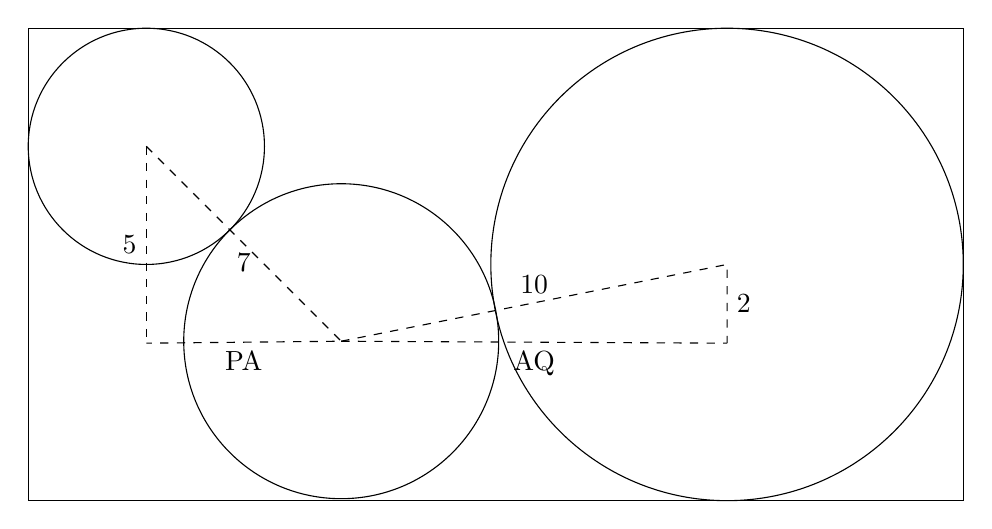
\begin{tikzpicture}[scale=0.5]
\draw (0,0)rectangle (17.75+6,-12);
\draw  (3,-3) circle (3);
\draw  (3,-3)+(-45:7) circle (4);
\draw  [dashed](3,-3)--node [left]{5}+(-90:5) ;
\draw  [dashed](3,-3)--node[below] {7}+(-45:7)--node[below]{PA}+(0,-5);
\draw  [dashed](3,-3)+(-45:7)--node[above]{10}(17.75,-6)--node[right]{2}+(0,-2);
\draw [dashed](3,-3)+(-45:7)--node[below]{AQ}(17.75,-8);
\draw  (17.75,-6) circle (6);
\end{tikzpicture}
\end{center}
$PA=\sqrt{7^2-5^2}=\sqrt{49-25}=\sqrt{24}=2\sqrt{6}$

$AQ=\sqrt{10^2-2^2}=\sqrt{100-4}=\sqrt{96}=4\sqrt{6}$

$PQ=PA+AQ=2\sqrt{6}+4\sqrt{6}=6 \sqrt{6}\approx \fbox{14.7}$



\end{document}